\documentclass{beamer}
\usetheme{Madrid}

\usepackage{adjustbox}
\usepackage{booktabs}
\usepackage{tablefootnote}
\usepackage{threeparttable}
\usepackage{array}
\usepackage{graphicx}
\usepackage{svg}
\usepackage{xcolor}
\usepackage{pgfgantt}
\usepackage{eurosym}
\usepackage{hyperref}
\usepackage{dirtree}
\usepackage[most]{tcolorbox}

\graphicspath{{../img/}{img/}}

\title[Desarrollo de un Compilador de Ensamblador]{Desarrollo de un Compilador Genérico de Lenguaje Ensamblador para el Simulador CREATOR}
\author{Álvaro Guerrero Espinosa}
\date{Leganés, Julio 2025}

\AtBeginSection[]{\begin{frame}
    \frametitle{Tabla de Contenidos}
    \tableofcontents[currentsection]
\end{frame}}

\newcommand{\svgfigure}[2][.8] {
\includesvg[inkscapelatex=false,width=#1\textwidth]{#2.svg}
}

% Fix \url{} colors. Hyperref messes up the colors of other links
\let\oldurl=\url
\renewcommand{\url}[1]{{\color{blue}\oldurl{#1}}}
\let\oldhref=\href
\renewcommand{\href}[2]{{\color{blue}\oldhref{#1}{#2}}}

\begin{document}

    \frame{\titlepage}

    \begin{frame}{Tabla de Contenidos}
        \tableofcontents
    \end{frame}

    \section{Introducción}

    \begin{frame}{Motivación}
        \begin{itemize}
            \item Importancia de conocer el funcionamiento general de un
            computador y el lenguaje ensamblador
            \begin{itemize}
                \item Los lenguajes de alto nivel se construyen sobre los de
                bajo nivel
                \item Sus capacidades y restricciones determinan el coste de las
                diferentes abstracciones
            \end{itemize}
            \item Para su enseñanza se utilizan simuladores
            \begin{itemize}
                \item Necesitan un ensamblador
            \end{itemize}
        \end{itemize}
    \end{frame}

    \begin{frame}{CREATOR}
        \centering
        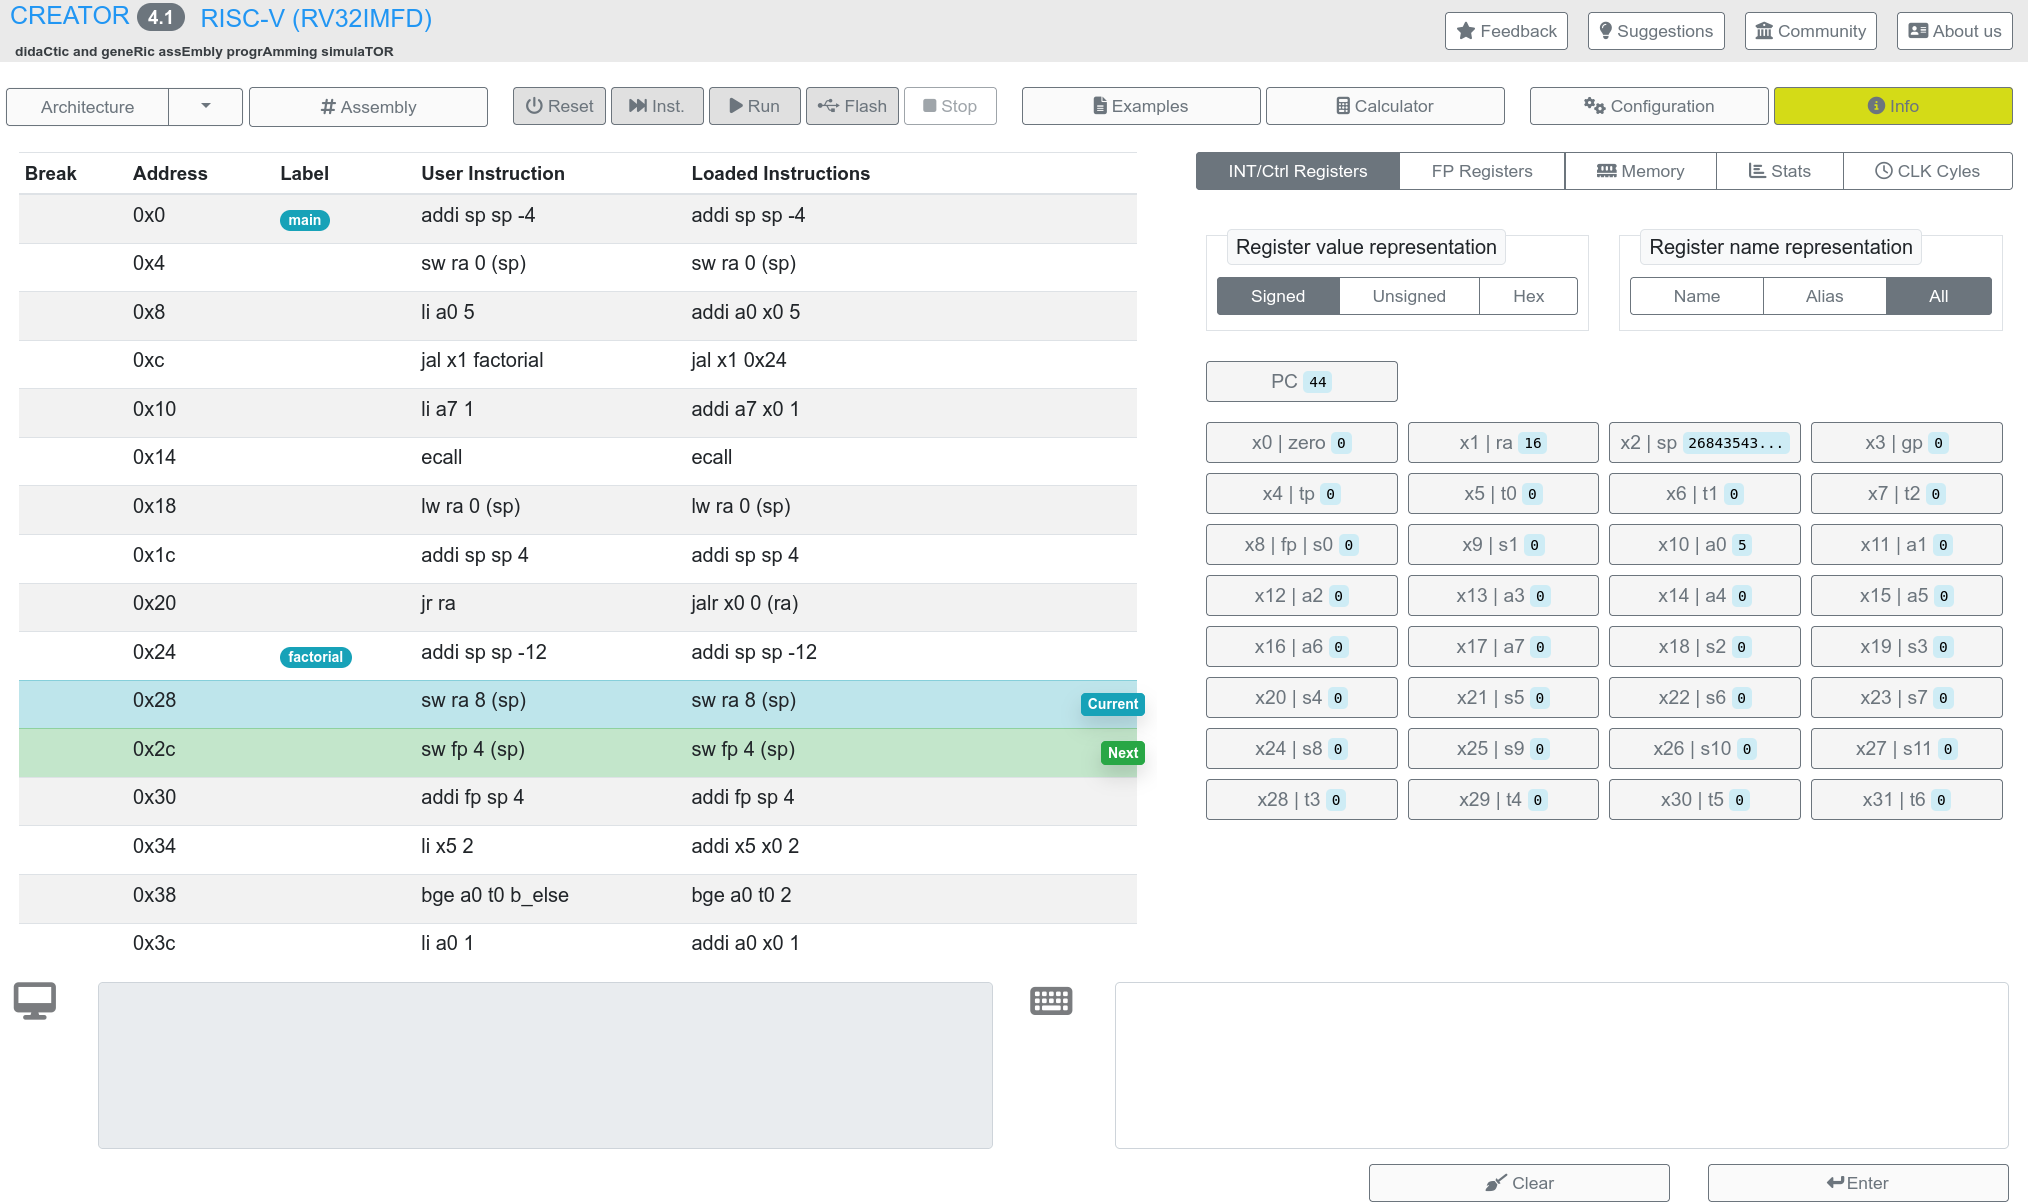
\includegraphics[width=0.9\textwidth]{creator}
        \url{https://creatorsim.github.io/}
    \end{frame}

    \begin{frame}{Objetivos}
        Desarrollar un ensamblador capaz de sustituir al actualmente utilizado
        por CREATOR corrigiendo sus problemas.

        \begin{itemize}
            \item Permitir funcionalidades avanzadas
            \item Mejorar los mensajes de error
            \item Organizar el código para facilitar su modificación
        \end{itemize}
    \end{frame}

    \section{Estado del arte}

    \begin{frame}{Ensambladores}
        \begin{itemize}
            \item Conversión de código ensamblador a una representación
            ejecutable
            \item Ejemplos: GNU Assembler (GAS), Tiny C Compiler Assembler
            (TCCASM), Netwide Assembler (NASM).\\~\\
        \end{itemize}

        \centering
        \begin{adjustbox}{max width=0.75\textwidth}
            \begin{threeparttable}[htb]
                \begin{tabular}{@{}>{\bfseries}lccccc@{}}
                    \toprule
                    Ensamblador              & GAS                 & TCCASM              & NASM                & CREATOR    & Propuesta    \\
                    \midrule                                                                                                 
                    Ejecución web            &                     &                     &                     & \checkmark & \checkmark \\
                    Biblioteca               &                     &                     &                     & \checkmark & \checkmark \\
                    Expresiones              & \checkmark\tnote{*} & \checkmark\tnote{*} & \checkmark\tnote{*} &            & \checkmark \\
                    Etiquetas como valores   & \checkmark          & \checkmark          & \checkmark          &            & \checkmark \\
                    Bigints                  & \checkmark          &                     &                     &            & \checkmark \\
                    UTF-8                    & \checkmark          & \checkmark          & \checkmark          &            & \checkmark \\
                    Definición de constantes & \checkmark          &                     & \checkmark          &            & \checkmark\tnote{**} \\
                    Macros                   & \checkmark          &                     & \checkmark          &            & \checkmark\tnote{**} \\
                    Compilación condicional  & \checkmark          &                     & \checkmark          &            & \checkmark\tnote{**} \\
                    Recuperación de errores  & \checkmark          &                     & \checkmark          &            & \checkmark\tnote{**} \\
                    \bottomrule
                \end{tabular}
                \begin{tablenotes}
                    \item [*] Solo posible con números enteros de tamaño fijo
                    \item [**] Trabajo futuro
                \end{tablenotes}
            \end{threeparttable}
        \end{adjustbox}
    \end{frame}

    \begin{frame}{Mensajes de error -- Ensambladores}
        \centering
        \svgfigure[0.7]{error_gas}

        GNU Assembler\\~\\

        \svgfigure[0.7]{error_tccasm}

        Tiny C Compiler Assembler\\~\\

        \svgfigure[0.7]{error_nasm}

        Netwide Assembler
    \end{frame}

    \begin{frame}{Mensajes de error -- Compiladores}
        \centering
        \svgfigure[0.9]{error_rust}
    \end{frame}

    \section{Análisis}

    \begin{frame}{Requisitos}
        \begin{columns}
            \column{0.41\textwidth}
            \begin{itemize}
                \item 19 Requisitos de usuario
                \begin{itemize}
                    \item 14 de capacidad
                    \item 5 de restricción
                \end{itemize}
                \item 40 Requisitos de software
                \begin{itemize}
                    \item 28 funcionales
                    \item 12 no funcionales
                \end{itemize}
            \end{itemize}

            \column{0.59\textwidth}
            \vspace{2mm}
            \begin{adjustbox}{max width=\textwidth}
                \begin{tabular}{@{}>{\bfseries}lp{8.1cm}@{}}
                    \toprule
                    RS-FN-08 & \\
                    \midrule
                    Descripción & El sistema debe soportar directivas de datos de números decimales con el formato IEEE 745 [48] de precisión simple (binary32) y doble (binary64). \\
                    Necesitdad & Esencial \\
                    Prioridad & Alta \\
                    Estabilidad & No cambia \\
                    Verificabilidad & Alta \\
                    Origen & RU-CA-01 \\
                    \bottomrule
                \end{tabular}
            \end{adjustbox}
        \end{columns}
    \end{frame}

    \section{Diseño}

    \begin{frame}{Funcionamiento}
        \centering
        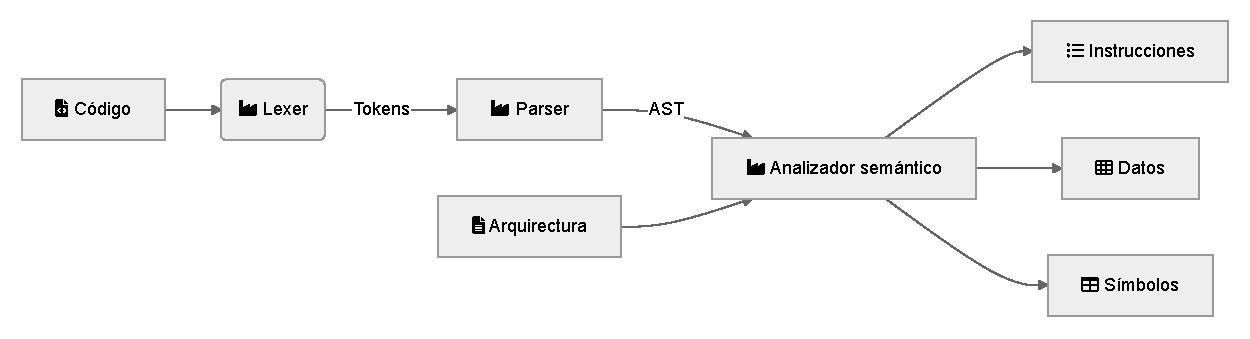
\includegraphics[width=1\textwidth]{funcionamiento}
    \end{frame}

    \begin{frame}{Arquitectura}
        \centering
        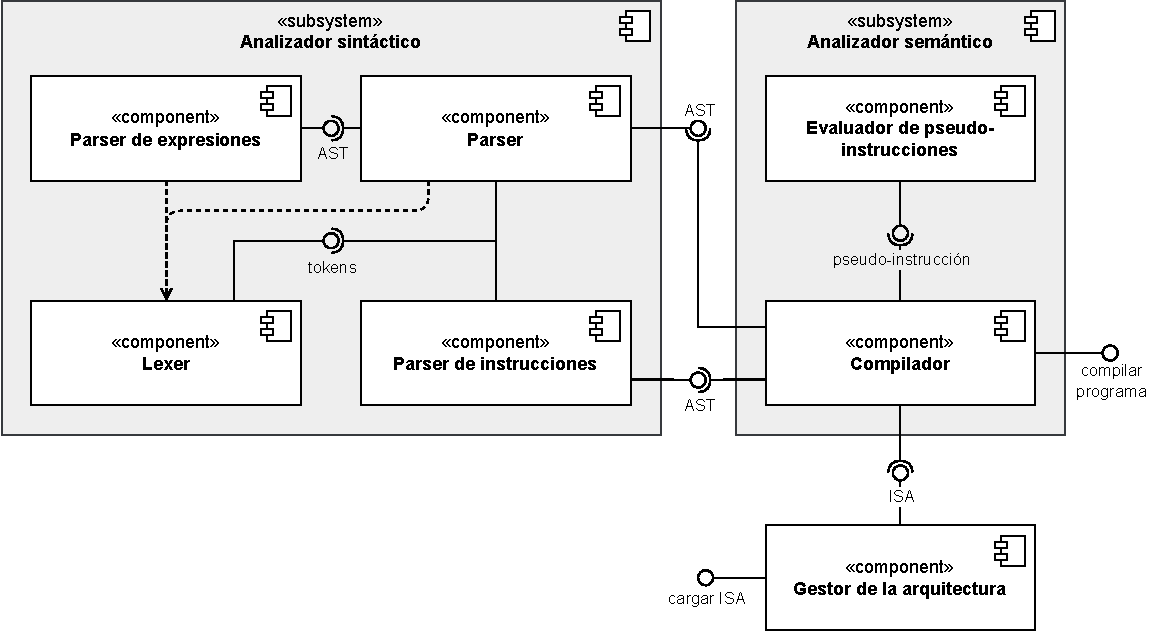
\includegraphics[width=0.9\textwidth]{components}
    \end{frame}

    \begin{frame}{Decisiones de diseño}
        \begin{itemize}
            \item Diseño modular
            \item Analizador sintáctico y semántico independientes
            \begin{itemize}
                \item AST como representación intermedia
            \end{itemize}
            \item Compilación de múltiples pasadas
            \item Rust y WebAssembly con una interfaz para JS
        \end{itemize}
    \end{frame}

    \begin{frame}{Mensajes de error}
        \begin{columns}
            \column{0.5\textwidth}
            \centering
            \svgfigure[1]{eval/1-new}
            \column{0.5\textwidth}
            \centering
            \svgfigure[1]{eval/3-new}
        \end{columns}
    \end{frame}

    \section{Implementación}

    \begin{frame}{Estructura de ficheros}
        \centering
        \begin{adjustbox}{max width=0.78\textwidth}
            \begin{tcolorbox}
                \dirtree{%
                    .1 /.
                    .2 js\_example/\DTcomment{Ejemplos de uso}.
                    .2 src/.
                    .3 architecture/\DTcomment{Deserialización de la arquitectura}.
                    .3 compiler/\DTcomment{Subsistema analizador semántico}.
                    .3 parser/\DTcomment{Subsistema analizador sintáctico}.
                    .3 architecture.rs\DTcomment{Gestor de la arquitectura}.
                    .3 compiler.rs\DTcomment{Traductor}.
                    .3 error\_rendering.rs\DTcomment{Renderizador de errores}.
                    .3 js.rs\DTcomment{API JS}.
                    .3 lib.rs\DTcomment{Biblioteca del compilador}.
                    .3 parser.rs\DTcomment{Parser}.
                    .3 span.rs\DTcomment{Región de código}.
                    .2 tests/\DTcomment{Arquitecturas de prueba}.
                    .2 Cargo.lock\DTcomment{Versiones de dependencias}.
                    .2 Cargo.toml\DTcomment{Metadatos de la biblioteca}.
                    .2 LICENSE.
                    .2 README.md.
                    .2 build.sh\DTcomment{Compilación biblioteca}.
                }
            \end{tcolorbox}
        \end{adjustbox}
    \end{frame}

    \section{Plan del proyecto}

    \begin{frame}{Tiempo estimado}
        \centering
        \begin{adjustbox}{max width=1\textwidth}
            \begin{ganttchart}[
                hgrid,
                time slot format=isodate,
                time slot unit=day,
                x unit=.06cm,
                y unit chart=0.4cm,
                y unit title=.7cm,
                title label font=\footnotesize,
                group label font=\bf\scriptsize,
                bar label font=\scriptsize,
                milestone label font=\it\scriptsize,
                vrule/.style={-},
            ]{2024-06-07}{2025-06-16}
                \gantttitlecalendar{year, month=shortname} \\

                \ganttgroup{I. Gestor de la arquitectura}{2024-06-07}{2024-06-30}\\
                \ganttbar{Planificación}{2024-06-07}{2024-06-09}\\
                \ganttlinkedbar{Análisis}{2024-06-10}{2024-06-12}\\
                \ganttlinkedbar{Desarrollo y pruebas}{2024-06-13}{2024-06-20}\\
                \ganttlinkedbar{Evaluación}{2024-06-21}{2024-06-24}\\
                \ganttlinkedbar{Documentación}{2024-06-24}{2024-06-30}\\

                \ganttgroup{II. Parser}{2024-07-01}{2024-09-09}\\
                \ganttbar{Planificación}{2024-07-01}{2024-07-03}\\
                \ganttlinkedbar{Análisis}{2024-07-04}{2024-07-17}\\
                \ganttlinkedbar{Desarrollo y pruebas}{2024-07-18}{2024-08-20}\\
                \ganttlinkedbar{Evaluación}{2024-08-21}{2024-08-31}\\
                \ganttlinkedbar{Documentación}{2024-09-01}{2024-09-09}\\

                \ganttgroup{III. Analizador semántico}{2024-09-10}{2024-12-20}\\
                \ganttbar{Planificación}{2024-09-10}{2024-09-14}\\
                \ganttlinkedbar{Análisis}{2024-09-15}{2024-09-25}\\
                \ganttlinkedbar{Desarrollo y pruebas}{2024-09-26}{2024-11-30}\\
                \ganttlinkedbar{Evaluación}{2024-12-01}{2024-12-09}\\
                \ganttlinkedbar{Documentación}{2024-12-10}{2024-12-20}\\

                \ganttgroup{IV. Integración con CREATOR}{2025-01-12}{2025-02-21}\\
                \ganttbar{Planificación}{2025-01-12}{2025-01-14}\\
                \ganttlinkedbar{Análisis}{2025-01-15}{2025-01-21}\\
                \ganttlinkedbar{Desarrollo y pruebas}{2025-01-22}{2025-02-08}\\
                \ganttlinkedbar{Evaluación}{2025-02-09}{2025-02-13}\\
                \ganttlinkedbar{Documentación}{2025-02-14}{2025-02-21}\\

                \ganttgroup{V. Pulido}{2025-02-22}{2025-04-20}\\
                \ganttbar{Planificación}{2025-02-22}{2025-02-24}\\
                \ganttlinkedbar{Análisis}{2025-02-25}{2025-02-28}\\
                \ganttlinkedbar{Desarrollo y pruebas}{2025-03-01}{2025-03-31}\\
                \ganttlinkedbar{Evaluación}{2025-04-01}{2025-04-10}\\
                \ganttlinkedbar{Documentación}{2025-04-11}{2025-04-18}\\

                \ganttgroup{Memoria}{2025-04-19}{2025-06-14}\\

                \ganttvrule{}{2025-01-01}

                % link iterations
                \ganttlink{elem0}{elem6}
                \ganttlink{elem6}{elem12}
                \ganttlink{elem12}{elem18}
                \ganttlink{elem18}{elem24}
                \ganttlink{elem24}{elem30}
            \end{ganttchart}
        \end{adjustbox}
    \end{frame}

    \begin{frame}{Presupuesto}
        \centering
        \begin{tabular}{lr}
            \toprule
            Personal          & 28.350,00 \euro \\
            Equipamiento      &    169,32 \euro \\
            Costes indirectos &    306,28 \euro \\
            \midrule
            \textbf{Total}    & \textbf{28.825,60 \euro} \\
            \bottomrule
        \end{tabular}
    \end{frame}

    \begin{frame}{Entorno socio-económico}
        \begin{itemize}
            \item Grandes empresas están empezando a diseñar procesadores
            propios
            \begin{itemize}
                \item Necesitan ingenieros con conocimiento de hardware y
                ensamblador
            \end{itemize}
            \item Usado por múltiples universidades españolas e internacionales
        \end{itemize}
    \end{frame}

    \section{Conclusiones y trabajos futuros}

    \begin{frame}{Concusiones}
        \begin{itemize}
            \item Ventajas del nuevo ensamblador
            \begin{itemize}
                \item Mejores mensajes de error
                \item Nuevas funcionalidades
                \item Código estructurado y flexible
            \end{itemize}
            \item Conocimientos adquiridos
            \begin{itemize}
                \item Diseño e implementación de compiladores y ensambladores
                \item Creación de interfaces entre lenguajes
                \item Programación en Rust
            \end{itemize}
        \end{itemize}
    \end{frame}

    \begin{frame}{Trabajos futuros}
        \begin{itemize}
            \item Más funcionalidades
            \begin{itemize}
                \item Macros
                \item Definición de constantes
                \item Compilación condicional
            \end{itemize}
            \item Estrategias de recuperación de errores
            \item Mejoras en la implementación
            \begin{itemize}
                \item Mejoras en la evaluación de expresiones
                \item Mejoras del \textit{parser}
            \end{itemize}
        \end{itemize}
    \end{frame}

    \begin{frame}{Demo}
        \begin{itemize}
            \item \href{https://creatorsim-community.github.io/creator-development/?architecture=RISC-V\%20(RV32IMFD)&asm=.data\%0Afunc_table\%3A\%20.word\%20f0\%2C\%20f1\%2C\%20f2\%2C\%20f3\%0A.text\%0Af0\%3A\%20mul\%20a0\%2C\%20a0\%2C\%20a1\%20\%23\%20a*b\%0A\%20\%20\%20\%20jr\%20ra\%0A\%0Af1\%3A\%20add\%20a0\%2C\%20a0\%2C\%20a1\%20\%23\%20a\%2Bb\%0A\%20\%20\%20\%20jr\%20ra\%0A\%0Af2\%3A\%20sub\%20a0\%2C\%20a0\%2C\%20a1\%20\%23\%20a-b\%0A\%20\%20\%20\%20jr\%20ra\%0A\%0Af3\%3A\%20mul\%20a0\%2C\%20a0\%2C\%20a1\%20\%23\%20(a*b)\%C2\%B2\%0A\%20\%20\%20\%20mul\%20a0\%2C\%20a0\%2C\%20a0\%0A\%20\%20\%20\%20jr\%20ra\%0A\%0Amain\%3A\%20loop\%3A\%0A\%20\%20\%20\%20\%20\%20li\%20a7\%2C\%205\%20\%20\%20\%20\%20\%20\%20\%20\%20\%20\%23\%20Ask\%20for\%20int\%20(function)\%0A\%20\%20\%20\%20\%20\%20ecall\%0A\%20\%20\%20\%20\%20\%20li\%20t1\%2C\%204\%0A\%20\%20\%20\%20\%20\%20mul\%20a0\%2C\%20a0\%2C\%20t1\%20\%20\%20\%20\%23\%20Multiply\%20by\%20word\%20size\%0A\%20\%20\%20\%20\%20\%20li\%20t0\%2C\%20func_table\%20\%23\%20Load\%20function\%20table\%20address\%0A\%20\%20\%20\%20\%20\%20add\%20t0\%2C\%20t0\%2C\%20a0\%20\%20\%20\%20\%23\%20Calculate\%20table\%20offset\%0A\%20\%20\%20\%20\%20\%20lw\%20t0\%2C\%200(t0)\%20\%20\%20\%20\%20\%20\%23\%20Load\%20the\%20table\%20value\%20(function\%20pointer)\%0A\%20\%20\%20\%20\%20\%20li\%20a0\%2C\%202\%0A\%20\%20\%20\%20\%20\%20li\%20a1\%2C\%203\%0A\%20\%20\%20\%20\%20\%20jalr\%20ra\%2C\%200(t0)\%20\%20\%20\%20\%23\%20Call\%20function\%0A\%20\%20\%20\%20\%20\%20li\%20a7\%2C\%201\%0A\%20\%20\%20\%20\%20\%20ecall\%20\%20\%20\%20\%20\%20\%20\%20\%20\%20\%20\%20\%20\%23\%20Print\%20result\%0A\%20\%20\%20\%20\%20\%20li\%20a0\%2C\%20'\%5Cn'\%0A\%20\%20\%20\%20\%20\%20li\%20a7\%2C\%2011\%0A\%20\%20\%20\%20\%20\%20ecall\%20\%20\%20\%20\%20\%20\%20\%20\%20\%20\%20\%20\%20\%23\%20Print\%20new\%20line\%0A\%20\%20\%20\%20\%20\%20j\%20loop\%20\%20\%20\%20\%20\%20\%20\%20\%20\%20\%20\%20\%23\%20Repeat}{Tabla de punteros}
        \end{itemize}
    \end{frame}
\end{document}
